
%(BEGIN_QUESTION)
% Copyright 2006, Tony R. Kuphaldt, released under the Creative Commons Attribution License (v 1.0)
% This means you may do almost anything with this work of mine, so long as you give me proper credit

En vanlig analysemåler for å detektere potensielt eksplosive gasser (ofte kalt en {\it LEL-analysator}, fra ``Lower Explosive Limit'') er en {\it katalytisk brennbar-gassensor}. I denne sensortypen varmes en tynn platinatråd opp av elektrisk strøm og dekkes med et katalytisk stoff. Hvis en blanding av brennbar gass og luft kommer i kontakt med sensoren, vil den påfølgende forbrenningen øke temperaturen i platinatråden. Da øker trådens motstand, og dette signaliserer tilstedeværelse av potensielt eksplosiv gass.

I denne spesifikke LEL-analysatoren er to identiske platinatrådsensorer koblet i serie: én eksponeres for en kontinuerlig strøm av prøvegass, mens den andre er forseglet slik at gass ikke når den. Spenningsfallene over disse to motstandselementene digitaliseres av to analog-til-digital-omformere (ADC-er) og tolkes av en mikrokontroller:

$$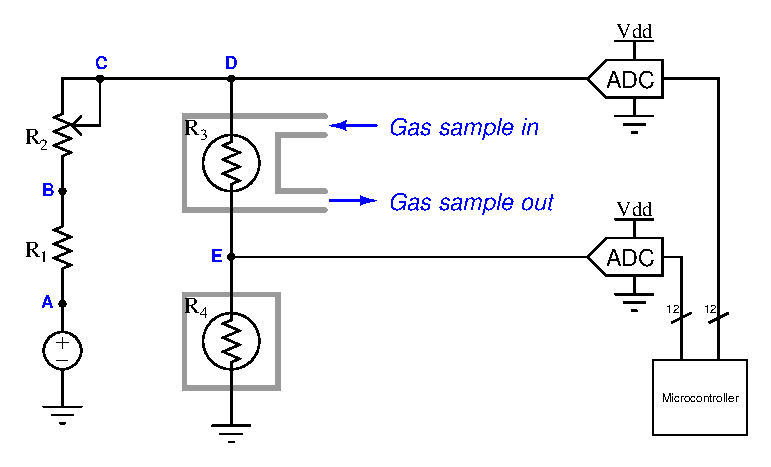
\includegraphics[width=15.5cm]{i01592x01.eps}$$

Anta at kretsen har en feil (den signaliserer eksplosiv gass selv når ingen gass er til stede). Hvor ville du startet med diagnostiske målinger for å isolere feilens art? Under hvilke prøvegassforhold ville du foretrukket å gjøre disse målingene, og hvorfor?

\vskip 20pt \vbox{\hrule \hbox{\strut \vrule{} {\bf Forslag til sokratisk diskusjon} \vrule} \hrule}

\begin{itemize}
\item{} Hvorfor tror du de to katalytiske trådsensorene er koblet i {\it serie}?
\item{} Hvilke elektriske måleverdier forventer du å se i en ``frisk'' krets, og hva kan du forvente å se i en krets der den aktive gassensoren har feilet?
\item{} Hvilke komponentfeil kan føre til at mikrokontrolleren ser et ``varmere'' signal for $R_3$ enn for $R_4$? Hvilken effekt vil dette ha på gassdeteksjonen?
\item{} Hvilke komponentfeil kan føre til at mikrokontrolleren ser et ``kaldere'' signal for $R_3$ enn for $R_4$? Hvilken effekt vil dette ha på gassdeteksjonen?
\item{} Hva ville skjedd dersom motstand $R_1$ feilet åpen?
\item{} Hva ville skjedd dersom motstand $R_1$ feilet kortsluttet?
\item{} Hva ville skjedd dersom variabelmotstand $R_2$ fikk lavere motstand?
\item{} Hva ville skjedd dersom variabelmotstand $R_2$ fikk høyere motstand?
\item{} Hvorfor tror du platinatråden i sensoren er belagt med en {\it katalysator}?
\item{} Denne typen LEL-sensor er avhengig av oksygeninnholdet i gassprøven. Bestem hvordan oksygenkonsentrasjonen påvirker analysatoren (dvs. vil økt oksygenkonsentrasjon få instrumentet til å ``tro'' at det er {\it mer} eller {\it mindre} brennbar gass til stede?), og lag deretter en metode for å kompensere for denne interferensen.
\end{itemize}

\underbar{file i01592}
%(END_QUESTION)





%(BEGIN_ANSWER)

I en korrekt fungerende krets uten eksplosiv gass til stede vil $U_{R3} = U_{R4}$, eller $U_D = 2 U_E$. Jeg lar det være opp til deg å identifisere gode diagnostiske tester!

%(END_ANSWER)





%(BEGIN_NOTES)

I en korrekt fungerende krets uten eksplosiv gass til stede vil $U_{R3} = U_{R4}$, eller $U_D = 2 U_E$.

\vskip 10pt

Bruk et multimeter for å se om $U_{R3} = U_{R4}$. Hvis den aktive sensoren har feilet åpen, vil $U_{R3} >> U_{R4}$.

\vskip 10pt

En tilstand med $U_{R3} >> U_{R4}$ kan oppstå hvis $R_3$ feiler åpen {\it eller} hvis $R_4$ feiler kortsluttet. Neste diagnostiske måling etter at du har verifisert $U_{R3} >> U_{R4}$, er spenningsmåling over motstand $R_1$: hvis det er spenningsfall der, går det strøm i sløyfen, og det betyr at $R_4$ har feilet kortsluttet. Hvis det ikke er spenningsfall over $R_1$, går det ingen strøm i sløyfen, og det betyr at $R_3$ har feilet åpen.

\vskip 10pt

Når disse diagnostiske testene utføres, anbefales det å eksponere analysatoren for en prøve uten brennbare gasser, for best mulig å avdekke feilen. Siden problemet her er at analysatoren registrerer en eksplosiv tilstand selv når den ikke finnes, bør vi sette analysatoren i en tilstand der den ``oppfører seg feil'' for å få tydeligst mulig symptomer. Hvis det faktisk var eksplosive gasser til stede under testene, kunne det blitt vanskelig å skille falske tegn på eksplosiv tilstand fra ekte tegn.

Som analogi: tenk på en bilmekaniker som får beskjed om at en bil lager en bestemt skranglelyd ved en bestemt hastighet. Ved feilsøking er det klokt å forsøke å gjenskape symptomet ved å kjøre bilen i den hastigheten og lytte til selve lyden (frekvens, plassering og amplitude). Å teste bilen i ro vil sjelden avsløre feilen, med mindre man er heldig.





\vskip 20pt \vbox{\hrule \hbox{\strut \vrule{} {\bf Virtuell feilsøking} \vrule} \hrule}

Denne oppgaven egner seg godt som øvelse i ``Virtuell feilsøking''. Presenter diagrammet for studentene, og tenk deg først en bestemt feil i systemet. Deretter presenterer du ett eller flere symptomer på feilen (noe en operatør eller annen bruker kan observere). Studentene foreslår så ulike diagnostiske tester for å finne feiltype og feilplassering, som om de var teknikere i en feilsøkingssituasjon. Din oppgave er å fortelle hva resultatet ville blitt for hver foreslått test, og dokumentere resultatene slik at alle studentene ser dem.

Under og etter øvelsen er det nyttig å stille oppfølgingsspørsmål som:

\begin{itemize}
\item{} Hva forteller resultatet av den siste testen om feilen?
\item{} Anta at resultatet av den siste testen var annerledes. Hva ville det da fortalt om feilen?
\item{} Er den siste diagnostiske testen den beste vi kunne gjort?
\item{} Hva ville vært ideell testrekkefølge for å diagnostisere problemet med færrest mulig steg?
\end{itemize}

%INDEX% Measurement, analytical: catalytic combustible gas sensor
%INDEX% Troubleshooting review: electric circuit diagnostic test usefulness

%(END_NOTES)
